\title{Introduzione}
\maketitle
\label{sec:intro}

\section{Cosa troverete in questo testo}
Bla bla bla qui spiego un po' come ho organizzato il testo ma questo lo faccio alla fine

\todo{finisci}


\section{Teoria del controllo}

\paragraph{È facile come andare in bicicletta.}
Questo proverbio viene spesso
usato quando si vuole sottolineare che un certo compito è \emph{molto facile}.
Infatti, sin da bambini, si può imparare ad usare la bicicletta con facilità e,
al giorno d'oggi, la maggior parte degli italiani\cite{https://www.ipsos.com/sites/default/files/ct/news/documents/2022-05/Ipsos\%20-\%20Cycling\%20Across\%20the\%20World-2022.pdf}
sa andare in bici.
Tuttavia, indagando più in profondità, si scopre che la matematica che ci
permette di svolgere un compito così semplice non è affatto banale\cite{a}.
Infatti, a differenza di ciò che spesso si pensa, non è sufficiente affidarsi
all'effetto giroscopico delle ruote per rimanere stabili, ma bisogna attivamente
\emph{controllare} la bici, agendo sul manubrio e spostando il proprio peso corporeo.
La moderna \emph{Teoria del Controllo} è la scienza che ci permette di studiare
analiticamente fenomeni di questo tipo, riconciliando la dualità che spesso
si osserva nella forma di \emph{compito-facile $\iff$ matematica-non-banale}.

\paragraph{La necessità di avere Controllo} è ampiamente diffusa in Natura\cite[b].
Basti pensare che tutti gli organismi viventi necessitano di meccanismi per controllare
il proprio metabolismo.
Meccanismi diversi permettono al singolo organismo di muoversi e agire secondo le sue decisioni.
Altri meccanismi regolano l'interazione tra organismi diversi della stessa specie.
Tutti questi fenomeni di natura diversa possono essere studiati tramite la stessa
formulazione matematica.

Per fissare le idee, consideriamo un sistema fisico descritto dall'equazione
\begin{equation*}
    \b A( \b y) = \b f( \b u)
\end{equation}
. $\b y \in Y$ è lo \emph{stato} e appartiene a uno spazio vettoriale
$Y$. $u \in \mathcal U_a$ è il \emph{controllo} e appartiene all'insieme dei
\emph{controlli ammissibili} $\mathcal U_a$.
\todo{bla bla ricopia paper storia swag fino a subito prima parte di feedback}
\todo{magari riscrivi col formalismo del brunton che è un po' più generale e bellino}


\subsection{Tipi di controllo}
\label{subsec:classificazione-dei-controlli}
Esistono diversi tipi di controllo. La scelta di quale strategia
usare dipende dal sistema che si sta studiando e dal risultato che si vuole
ottenere.
Per fissare le idee, prendiamo come esempio un problema di controllo che è
comune a tutti -- il traffico -- e andiamo a vedere quali strategie possiamo
usare per affrontarlo applicare.

\paragraph{Il controllo passivo} è una strategia che non usa alcun tipo di
risorsa dinamica -- ovvero, di energia--.
I segnali stradali sono un ottimo esempio: una volta installati, non necessitano
di alcuna risorsa per operare.
Tuttavia, se le condizioni della strada sono variabili, è necessario
introdurre un modo di variare i controlli. Abbiamo quindi diversi tipi
di \emph{controllo attivo}.

\paragraph{Il controllo attivo} ha bisogno di energia per funzionare e può fare
uso di \emph{sensori}.
Si distinguono principalmente due categorie di sistemi controllati attivamente:
\emph{open-loop} e \emph{closed-loop}. Open-loop sono i sistemi in cui viene
applicato un controllo che \emph{non dipende} dallo stato del sistema stesso,
mentre quelli closed-loop usano lo stato del sistema misurato
per decidere quale controllo applicare nell'istante di tempo successivo alla misura.
Trovo che il modo più intuitivo di spiegare questa distinzione sia tramite uno
schema (figura \ref{fig:open-vs-closed}).
Nel contesto del traffico, un sistema di controllo attivo è dato dai semafori;
questi possono operare open-loop -- accendendosi e spegnendosi con
frequenze programmate -- oppure closed-loop -- usando sensori per misurare il volume del traffico --.

Esistono infine dei casi in cui i sensori non vengono usati per misurare
lo stato del sistema, ma \emph{ne misurano i disturbi esterni} e applicano un
controllo preventivo. Basti pensare a cosa succede quando si verifica un incidente
in autostrada: il traffico viene rallentato e dirottato ancora prima che i soccorsi
chiudano la strada.

\paragraph{}
Una suddivisione schematica di queste categorie è riportata in figura \ref{fig:control-types}.
In questo testo tratterò solamente di alcune strategie di controllo. In particolare,
mi concentrerò sul controllo closed-loop applicato a sistemi lineari.

\begin{figure}[thb]
    \centering
    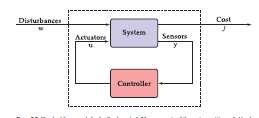
\includegraphics[width=0.4\textwidth]{assets/open-vs-closed.png}
    \caption{controllo }%todo
    \label{fig:open-vs-closed}
\end{figure}


\begin{figure}[thb]
    \centering
    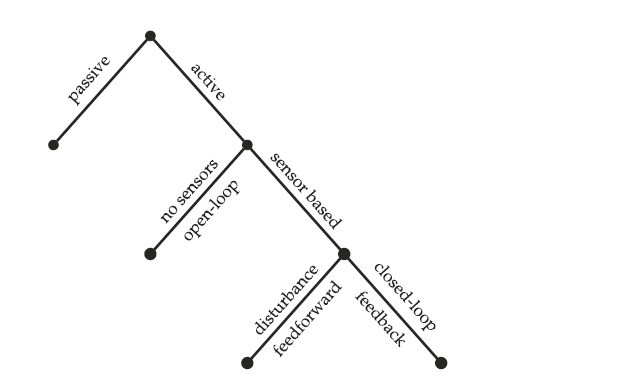
\includegraphics[width=0.4\textwidth]{assets/control-types.png}
    \caption{Schematic illustrating the various types of control.} %todo tipi di controllo}
    \label{fig:control-types}
\end{figure}

\subsection{Controllo ottimale}
\label{subsec:controllo-ottimale}
Qui parlo un attimo dei criteri che si usano per scegliere il controllo e di
cosa userò io.

\subsection{Sistemi lineari}
E qui secondo me ci sta una brevissima introduzione su cosa vuol dire
controllare un sistema lineare (vs non lineare).

\section{Il "doppio pendolo invertito su rotaia"}
Qui spiego come mai ho scelto questo sistema

\subsection{Modello del sistema}
Qui parlo brevemente di come ho trovato le equazioni e di come ho ridotto l'ordine
del problema aumentando la dimensione dello spazio delle fasi

\subsection{Realizzazione del sistema nel mondo reale}
Flex